\documentclass{article}
\usepackage{amsmath}
\usepackage{amssymb}
\usepackage{xargs}
\usepackage[dvipsnames]{xcolor}
\usepackage[margin=1.2in]{geometry}
\usepackage{graphicx}
\usepackage{pgfplots, pgfplotstable}
\usetikzlibrary{datavisualization.formats.functions}
\usepgfplotslibrary{fillbetween}
\usetikzlibrary{patterns}
\usepackage{tikz}

\begin{document}

\title{Differential Equations HW \#2}
\author{Ozaner Hansha}
\date{October 3, 2019}
\maketitle

\newcommandx{\der}[2][1=y, 2=t]{\frac{d#1}{d#2}}
\newcommand*\eval[3]{\left[#1\right]_{#2}^{#3}}

\section*{Problem 1}
\noindent\textbf{Problem:} Given the following IVP:

% \[\begin{cases}
%     y'=t+y \\
%     y(0)=1
% \end{cases}\]

\begin{equation*}
    y'=t+y,\,\,\,\, y(0)=1
\end{equation*}

Given that the zeroth term of the Picard iteration is $y_0(t)=1$, calculate the next two terms $y_1(t),y_2(t)$.
\bigskip

\noindent\textbf{Solution:} Recall that the Picard iteration of an IVP is given by:

\begin{equation*}
    y_{n+1}=y_0+\int_{t_0}^t f(t,y_n)\mathop{dt}
\end{equation*}

And so the first iterate $y_1$ is given by:

\begin{align*}
    y_1(t)&=1+\int_0^t (t+1)\mathop{dt}\\
    &=1+\eval{\frac{t^2}{2}+t}{0}{t}\\
    &=\frac{t^2}{2}+t+1
\end{align*}

And the second iterate $y_2$ given by:

\begin{align*}
    y_2(t)&=1+\int_0^t \left(t+\frac{t^2}{2}+t+1\right)\mathop{dt}\\
    &=1+\int_0^t \left(\frac{t^2}{2}+2t+1\right)\mathop{dt}\\
    &=1+\eval{\frac{t^3}{6}+t^2+t}{0}{t}\\
    &=\frac{t^3}{6}+t^2+t+1
\end{align*}
\pagebreak

\section*{Problem 2}
\noindent\textbf{Problem:} Show that the following IVP does not have a solution $y(t)$ defined on any interval $(-\epsilon, \epsilon)$:

% Define the function $f$ as:

% \[f(t,y)=\begin{cases}
%     \frac{y}{t},&\text{if }t\not=0 \\
%     0,&\text{if }t=0
% \end{cases}\]

% \[\begin{cases}
%     y'=f(t,y) \\
%     y(0)=1
% \end{cases}\]
\begin{equation*}
    y'=\begin{cases}
        \frac{y}{t},&\text{if }t\not=0 \\
        0,&\text{if }t=0
    \end{cases},\,\,\,\,\,\,\,\, y(0)=1
\end{equation*}

\noindent\textbf{Solution:} We can see that for $t\not=0$ this is a separable equation, and so its solution set is given by:
\begin{align*}
    \der&=\frac{y}{t}\\
    \int \frac{1}{y}\mathop{dy}&=\int \frac{1}{t}\mathop{dt}\tag{separable equation}\\
    \ln{|y|}&=\ln{|t|}+C_1\tag{integration}\\
    |y|&=e^{C_1}|t|\tag{exponentiation}\\
    y&=C_2t\tag{$\pm e^{C_1}=C_2\not=0$}
\end{align*}

Note that by letting $C_2=0$, we arrive at what happens to be the equation's sole equilibrium solution: $y=0$. Thus we can replace $C_2$ with a new constant $C_3$ that can take on any real value. This gives us the following family of solutions indexed by $C_3\in\mathbb R$:

\begin{equation*}
    y_{C_3}(t)=C_3t
\end{equation*}

Note, however, that there is no constant $C_3$ that can satisfy the initial condition:

\begin{equation*}
    (\forall C_3\in\mathbb R)\,\,y_{C_3}(0)=C_3\cdot0\not=1
\end{equation*}

And so the initial condition can't be satisfied by any solution of the differential equation.

\section*{Problem 3}
\noindent\textbf{Part a:} Sketch the phase line of the following autonomous equation:

\begin{equation*}
    y'=\sin y,\,\,\,\,\,\,\,\,\,\,\,\,\,\, y\in(-3\pi,3\pi)
\end{equation*}

\noindent\textbf{Solution:} The equilibrium points of the differential equation are given by the roots of $\sin y$ which are just the integer multiples of $\pi$ (within the given domain):

\begin{equation*}
    (\forall n\in\mathbb N)\,\,y'(n\pi)=\sin(n\pi)=0
\end{equation*}

Now we apply the first derivative test to classify these equilibria as either sources or sinks:

\begin{equation*}
    \der[][y]\sin (n\pi)=\cos(n\pi)=(-1)^{n}
\end{equation*}

This is to say that for even $n$ the equilibrium point is a source, and for odd $n$ it's a sink. We now have enough information to draw our phase line, complete with equilibria and decreasing/increasing intervals:

\begin{center}
    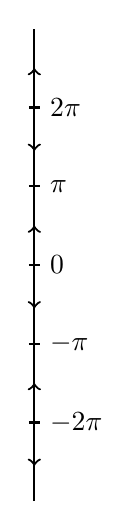
\begin{tikzpicture}[thick]
    \gdef\AxisMin{-3}
    \gdef\AxisMax{3}
    %Equilibria
    \draw  (-2pt,-2) -- (2pt,-2) node [right] {$-2\pi$};
    \draw  (-2pt,-1) -- (2pt,-1) node [right] {$-\pi$};
    \draw  (-2pt,0) -- (2pt,0) node [right] {$0$};
    \draw  (-2pt,2) -- (2pt,2) node [right] {$2\pi$};
    \draw  (-2pt,1) -- (2pt,1) node [right] {$\pi$};
    %Up
    \draw [<-] (0,-0.5-0.05) -- (0,-0.5);
    \draw [<-] (0,1.5-0.05) -- (0,1.5);
    \draw [<-] (0,-2.5-0.05) -- (0,-2.5);
    
    %Down
    \draw [->] (0,0.5-0.05) -- (0,0.5);
    \draw [->] (0,-1.5-0.05) -- (0,-1.5);
    \draw [->] (0,2.5-0.05) -- (0,2.5);

    \draw  (0,-3) -- (0,3);
    \end{tikzpicture}
\end{center}

% Notice that we included the equilibrium points $y=\pm3\pi$. This si because, despite not being in the domain, all solutions in the interval

\noindent\textbf{Part b:} Sketch the phase line of the following autonomous equation:

\begin{equation*}
    y'=f(y)=y^3+2y^2-y
\end{equation*}

\noindent\textbf{Solution:} The equilibrium points are given by the roots of the differential equation:

\begin{align*}
    f(y)=y^3+2y^2-y&=0\\
    y(y^2+2y-1)&=0\\
    y(y+\sqrt{2}+1)(y-\sqrt{2}+1)&=0\\
    y&=0,\pm\sqrt{2}-1
\end{align*}

Now we apply the first derivative test to classify these equilibria as either sources or sinks:
\medskip
\begin{align*}
    f'(y)&=3y^2+4y-1\\
    f'(0)&=3\cdot0^2+4\cdot0-1=-1<0\\
    f'(\sqrt{2}-1)&=3(\sqrt{2}-1)^2+4(\sqrt{2}-1)-1=4-2\sqrt{2}>0\\
    f'(-\sqrt{2}-1)&=3(-\sqrt{2}-1)^2+4(-\sqrt{2}-1)-1=4+2\sqrt{2}>0
\end{align*}

And so 0 is sink, and $\pm\sqrt{2}-1$ are sources. We now have enough information to draw our phase line:

\begin{center}
    \begin{tikzpicture}[thick]
    \gdef\AxisMin{-3}
    \gdef\AxisMax{2}
    %Equilibria
    \draw  (-2pt,-2.41421) -- (2pt,-2.41421) node [right] {$-\sqrt{2}-1$};
    \draw  (-2pt,0.41421+1) -- (2pt,0.41421+1) node [right] {$\sqrt{2}-1$};
    \draw  (-2pt,0+1) -- (2pt,0+1) node [left] {$0\,\,\,\,$};
    
    %Up
    \draw [<-] (0,1.245-0.05) -- (0,1.245);
    \draw [<-] (0,-2.7-0.05) -- (0,-2.7);
    
    %Down
    \draw [->] (0,-1.2071-0.05+.5) -- (0,-1.2071+.5);
    \draw [->] (0,1.245+.5-0.05) -- (0,1.245+.5);

    \draw  (0,-3) -- (0,2);
    \end{tikzpicture}
\end{center}

\section*{Problem 4}
\noindent\textbf{Part a:} Sketch the bifurcation diagram of the following family of autonomous differential equations, and identify all bifurcation values:

\begin{equation*}
    y'=f_\mu(y)=4y^2+\mu^2-1
\end{equation*}

\noindent\textbf{Solution:} The bifurcation diagram is simply the graph found by setting the family equal to 0, and solving for $y$ in terms of the parameter $\mu$:

\begin{align*}
    y'=4y^2+\mu^2-1&=0\\
    4y^2&=1-\mu^2\\
    y^2&=\frac{1-\mu^2}{4}\\
    y&=\frac{\pm\sqrt{1-\mu^2}}{2}\\
\end{align*}

To shade in the decreasing/increasing sectors, we test $\mu=0$ giving us the following equilibria:

\begin{equation*}
    y=\frac{\pm\sqrt{1-0^2}}{2}=\frac{\pm\sqrt{1}}{2}=\pm\frac{1}{2}
\end{equation*}

Performing the first derivative test on these equilibria tells us:

\begin{align*}
    f_0'(y)&=8y\\
    f_0'\left(\frac{1}{2}\right)&=8\cdot\frac{1}{2}=4>0\\
    f_0'\left(-\frac{1}{2}\right)&=8\cdot\frac{-1}{2}=-4<0
\end{align*}

Which tells us that $\frac{1}{2}$ is a source and $-\frac{1}{2}$ is a sink. We now have enough information to graph and shade the bifurcation diagram:

\begin{center}
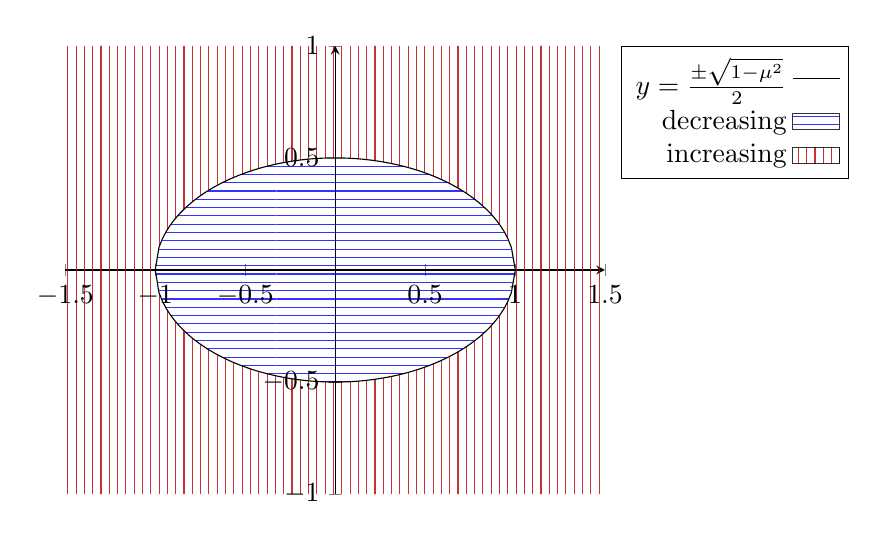
\begin{tikzpicture}
    \begin{axis}[
        xmin=-1.5,xmax=1.5,
        ymin=-1,ymax=1,
        legend pos=outer north east,
        axis lines=center,
        legend style={legend cell align=right,legend plot pos=right}]
    
    \addplot[color=black,domain=-1:1,samples=100] {(sqrt(1-x^2))/2};
    \addplot[color=black,domain=-1:1,samples=100,forget plot] {-(sqrt(1-x^2))/2};
    \addlegendentry{$y=\frac{\pm\sqrt{1-\mu^2}}{2}$}

    \plot[name path=A, thick,samples=100,domain=-1:1,
        forget plot,draw=none] {(sqrt(1-x^2))/2};
    \plot[name path=B,thick,samples=100,domain=-1:1,
        forget plot,draw=none] {-(sqrt(1-x^2))/2};
    \addplot[fill=blue,
        opacity=.8,
        pattern=horizontal lines,
        pattern color=blue]
        fill between [of=A and B, soft clip={domain=-1:1}];
    % \addlegendentry{$0\le y\le\frac{x}{2}$}
    \addlegendentry{decreasing}
    
    \plot[name path=C, thick,samples=100,domain=-1.5:1.5,
        forget plot,draw=none] {1};
    \plot[name path=D,thick,samples=100,domain=-1.5:1.5,
        forget plot,draw=none] {-1};
    \plot[name path=E,thick,samples=100,domain=-1.5:1.5,
        forget plot,draw=none] {0};
    \addplot[fill=BrickRed,
        opacity=.8,
        pattern=vertical lines,
        pattern color=BrickRed]
        fill between [of=B and D, soft clip={domain=-1:1}];
    \addplot[fill=BrickRed,
        opacity=.8,
        pattern=vertical lines,
        pattern color=BrickRed]
        fill between [of=E and D, soft clip={domain=-1.5:-1}];
    \addplot[fill=BrickRed,
        opacity=.8,
        pattern=vertical lines,
        pattern color=BrickRed]
        fill between [of=E and D, soft clip={domain=1:1.5}];
        
    \addplot[fill=BrickRed,
        opacity=.8,
        pattern=vertical lines,
        pattern color=BrickRed]
        fill between [of=A and C, soft clip={domain=-1:1}];
    \addplot[fill=BrickRed,
        opacity=.8,
        pattern=vertical lines,
        pattern color=BrickRed]
        fill between [of=E and C, soft clip={domain=-1.5:-1}];
    \addplot[fill=BrickRed,
        opacity=.8,
        pattern=vertical lines,
        pattern color=BrickRed]
        fill between [of=E and C, soft clip={domain=1:1.5}];
    \addlegendentry{increasing}

    \end{axis}
\end{tikzpicture}
\end{center}

We can clearly see that a change in the number of equilibria occurs when $\mu=\pm 1$, and so these are our bifurcation values.
\bigskip

\noindent\textbf{Part b:} Sketch the bifurcation diagram of the following family of autonomous differential equations, and identify all bifurcation values:

\begin{equation*}
    y'=f_\mu(y)=(y-1)(y^2-\mu^2)
\end{equation*}

\noindent\textbf{Solution:} The bifurcation diagram is the set of all points $(y,\mu)$ such that $y$ is an equilibrium point of $f_\mu(y)=0$. Examining the differential equation, we see that $y=1$ will always be an equilibrium point:

\begin{equation*}
    (\forall\mu\in\mathbb R)\,\,f_\mu(1)=(1-1)(1^2-\mu^2)=0
\end{equation*}

To find the other equilibria, we simply set the other factor equal to 0 and solve for $y$:
\begin{align*}
    y^2-\mu^2&=0\\
    y^2&=\mu^2\\
    y&=\pm\mu
\end{align*}

To shade in the decreasing/increasing sectors, we first copmute the derivative of $f_\mu(y)$:

\begin{equation*}
    f_\mu'(y)=3y^2-2y-\mu^2
\end{equation*}

Now we test $\mu=\frac{1}{2}$ giving us the following:

\begin{align*}
    f_\frac{1}{2}(y)&=0\implies y=1,\pm\frac{1}{2}\\
    f_\frac{1}{2}\left(\frac{1}{2}\right)&=\frac{3}{4}-1-\frac{1}{4}=-\frac{1}{2}<0\\
    f_\frac{1}{2}\left(-\frac{1}{2}\right)&=\frac{3}{4}+1-\frac{1}{4}=\frac{3}{2}>0\\
    f_\frac{1}{2}(1)&=3-2-\frac{1}{4}=\frac{3}{4}>0
\end{align*}

And so we have $\frac{1}{2}$ is a sink, and $1,-\frac{1}{2}$ are sources. For the remaining regions, we test $\mu=2$ giving us the following:
\begin{align*}
    f_2(y)&=0\implies y=1,\pm2\\
    f_2(2)&=12-4-4=4>0\\
    f_2(-2)&=12+4-4=12>0\\
    f_2(1)&=3-2-4=-3<0
\end{align*}

And so we have $1$ is a sink, and $\pm 2$ are sources. We now have enough information, thanks to symmetry, to graph and shade the bifurcation diagram:

\begin{center}
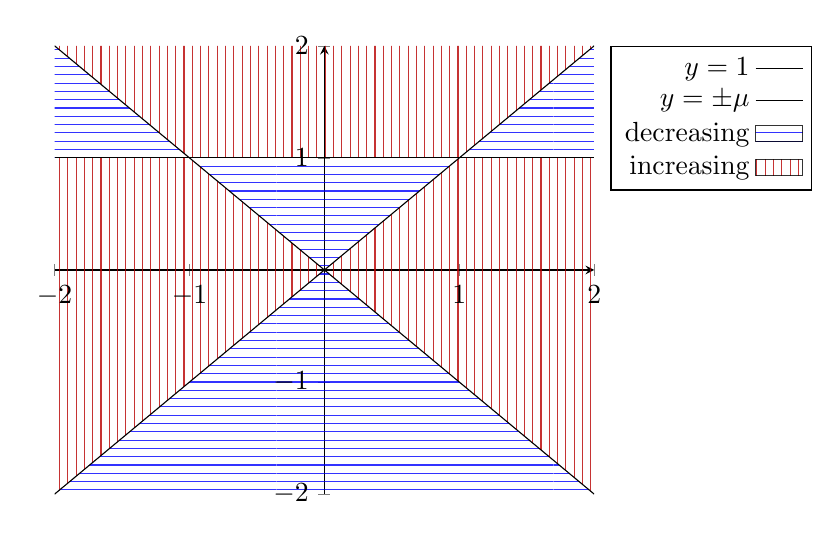
\begin{tikzpicture}
    \begin{axis}[
        xmin=-2,xmax=2,
        ymin=-2,ymax=2,
        axis lines=center,
        legend pos=outer north east,
        legend style={legend cell align=right,legend plot pos=right}]
    
    \addplot[color=black,domain=-2:2,samples=200] {1};
    \addplot[color=black,domain=-2:2,samples=100] {-x};
    \addplot[color=black,domain=-2:2,samples=100,forget plot] {x};
    \addlegendentry{$y=1$}
    \addlegendentry{$y=\pm\mu$}

    \plot[name path=A, thick,samples=100,domain=-2:2,
        forget plot,draw=none] {1};
    \plot[name path=B,thick,samples=100,domain=-2:2,
        forget plot,draw=none] {x};
    \plot[name path=C, thick,samples=100,domain=-2:2,
        forget plot,draw=none] {-x};
    \plot[name path=D, thick,samples=100,domain=-2:2,
        forget plot,draw=none] {2};
    \plot[name path=E, thick,samples=100,domain=-2:2,
        forget plot,draw=none] {-2};
    \addplot[fill=blue,
        opacity=.8,
        pattern=horizontal lines,
        pattern color=blue]
        fill between [of=B and E, soft clip={domain=-2:0}];
    \addplot[fill=blue,
        forget plot,
        opacity=.8,
        pattern=horizontal lines,
        pattern color=blue]
        fill between [of=C and E, soft clip={domain=0:2}];
    \addplot[fill=blue,
        forget plot,
        opacity=.8,
        pattern=horizontal lines,
        pattern color=blue]
        fill between [of=B and A, soft clip={domain=0:2}];
    \addplot[fill=blue,
        forget plot,
        opacity=.8,
        pattern=horizontal lines,
        pattern color=blue]
        fill between [of=C and A, soft clip={domain=-2:0}];
    \addlegendentry{decreasing}
        
    \addplot[fill=BrickRed,
        opacity=.8,
        pattern=vertical lines,
        pattern color=BrickRed]
        fill between [of=B and A, soft clip={domain=-2:-1}];
    \addplot[fill=BrickRed,
        forget plot,
        opacity=.8,
        pattern=vertical lines,
        pattern color=BrickRed]
        fill between [of=C and A, soft clip={domain=1:2}];
    \addplot[fill=BrickRed,
        forget plot,
        opacity=.8,
        pattern=vertical lines,
        pattern color=BrickRed]
        fill between [of=B and C, soft clip={domain=-1:1}];
    \addplot[fill=BrickRed,
        opacity=.8,
        pattern=vertical lines,
        pattern color=BrickRed]
        fill between [of=C and D, soft clip={domain=-2:-1}];
    \addplot[fill=BrickRed,
        forget plot,
        opacity=.8,
        pattern=vertical lines,
        pattern color=BrickRed]
        fill between [of=B and D, soft clip={domain=1:2}];
    \addplot[fill=BrickRed,
        forget plot,
        opacity=.8,
        pattern=vertical lines,
        pattern color=BrickRed]
        fill between [of=A and D, soft clip={domain=-1:1}];
    \addlegendentry{increasing}

    \end{axis}
\end{tikzpicture}
\end{center}

We can see that there are 3 equilibrium points for all values of $\mu$ except for $\mu=0,\pm1$ which all have 2 equilibria. And so these 3 values are the bifurcation values of the given autonomous family.

\section*{Problem 5}
\noindent\textbf{Problem:} Consider the following population model with harvesting:

\begin{equation}
    P'=kP\left(1-\frac{P}{N}\right)-\alpha P
\end{equation}

where $k, N > 0$ are fixed (that is, the harvesting rate is proportional to the total population). Find the critical value $\alpha_0$ so that the population will become extinct if $\alpha > \alpha_0$ (you may assume that the initial population is $N$).\bigskip

\noindent\textbf{Solution:} Let us first rewrite the differential equation like so:

\begin{equation}
    P'=kP\left(1-\alpha-\frac{P}{N}\right)
\end{equation}

As we can see, $P=0$ will always be an equilibrium point:

\begin{equation*}
    (\forall\alpha\in\mathbb R)\,\,P_\alpha'(0)=k\cdot0\cdot\left((1-\alpha-\frac{0}{N}\right)=0
\end{equation*}

To find the other equilibria, we simply set the other factor equal to 0 and solve for $y$:

\begin{align*}
    1-\alpha-\frac{P}{N}&=0\\
    \frac{P}{N}&=1-\alpha\\
    P&=N(1-\alpha)
\end{align*}

% Graphing these points we arrive at the following bifurcation diagram:

% \begin{center}
%     \begin{tikzpicture}
%         \begin{axis}[
%             xmin=-1,xmax=2,
%             yticklabels={$0$,$-N$,$2N$,$N$,$2N$},
%             ymin=-1.5,ymax=2,
%             axis lines=center,
%             legend pos=outer north east,
%             legend style={legend cell align=right,legend plot pos=right}]
        
%         \addplot[color=BrickRed,domain=-2:2,samples=200] {0};
%         \addplot[color=blue,domain=-2:2,samples=100] {1-x};
%         \addlegendentry{$y=0$}
%         \addlegendentry{$y=1-\alpha$}
%         \end{axis}
%     \end{tikzpicture}
%     \end{center}

To shade the decreasing/increasing sectors, we first test $\alpha=0$ giving us the following equation:

\begin{equation*}
    P_0'=kP\left(1-\frac{P}{N}\right)=kP-\frac{kP^2}{N}
\end{equation*}

Its equilibrium points are $P=0,N$. Now we just perform the first derivative test:

\begin{align*}
    \der[P_0'][P]=f_0'(P)&=k-\frac{2kP}{N}\\
    f_0'(0)&=k-0=k>0\\
    f_0'(N)&=k-2k=-k<0
\end{align*}

This tells us that 0 is a source, and $N$ a sink. And now for the remaining sector we test $\alpha=2$, giving us the following equation:

\begin{equation*}
    P_2'=kP\left(-1-\frac{P}{N}\right)=-kP-\frac{kP^2}{N}
\end{equation*}

Its equilibrium points are $P=0,-N$. Now we just perform the first derivative test:

\begin{align*}
    \der[P_2'][P]=f_2'(P)&=-k-\frac{2kP}{N}\\
    f_2'(0)&=-k-0=-k<0\\
    f_2'(-N)&=k+2k=k>0
\end{align*}

This tells us that 0 is a sink, and $-N$ a source. We now have enough information to graph the and shade the bifurcation diagram:

\begin{center}
    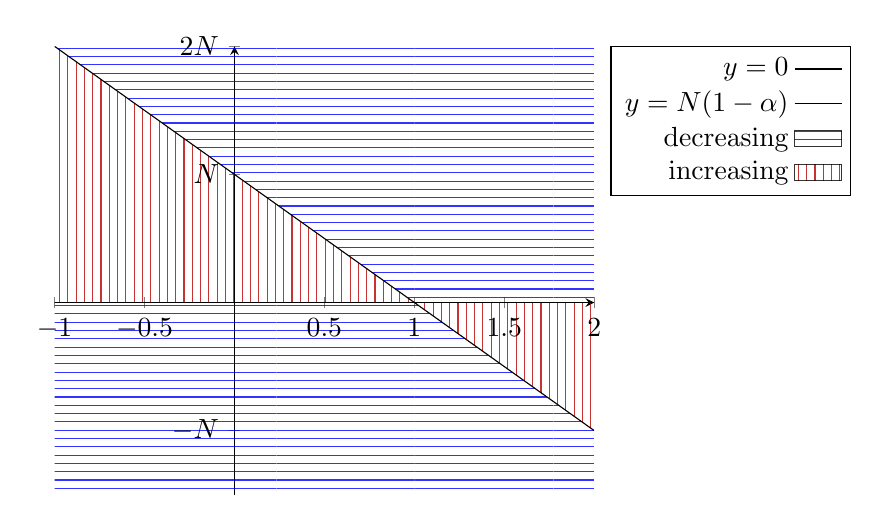
\begin{tikzpicture}
        \begin{axis}[
            xmin=-1,xmax=2,
            ymin=-1.5,ymax=2,
            axis lines=center,
            yticklabels={$0$,$-N$,$2N$,$N$,$2N$},
            legend pos=outer north east,
            legend style={legend cell align=right,legend plot pos=right}]
        
        \addplot[color=black,domain=-2:2,samples=200] {0};
        \addplot[color=black,domain=-2:2,samples=100] {1-x};
        \addlegendentry{$y=0$}
        \addlegendentry{$y=N(1-\alpha)$}
    
        \plot[name path=A, thick,samples=100,domain=-2:2,
            forget plot,draw=none] {0};
        \plot[name path=B,thick,samples=100,domain=-2:2,
            forget plot,draw=none] {1-x};
        \plot[name path=D, thick,samples=100,domain=-2:2,
            forget plot,draw=none] {2};
        \plot[name path=E, thick,samples=100,domain=-2:2,
            forget plot,draw=none] {-2};
        \addplot[fill=blue,
            opacity=.8,
            pattern=horizontal lines,
            pattern color=blue]
            fill between [of=A and E, soft clip={domain=-2:1}];
        \addplot[fill=blue,
            opacity=.8,
            forget plot,
            pattern=horizontal lines,
            pattern color=blue]
            fill between [of=B and E, soft clip={domain=1:2}];
        \addplot[fill=blue,
            opacity=.8,
            forget plot,
            pattern=horizontal lines,
            pattern color=blue]
            fill between [of=B and D, soft clip={domain=-2:1}];
        \addplot[fill=blue,
            opacity=.8,
            forget plot,
            pattern=horizontal lines,
            pattern color=blue]
            fill between [of=A and D, soft clip={domain=1:2}];
        \addlegendentry{decreasing}
            
        \addplot[fill=BrickRed,
            opacity=.8,
            pattern=vertical lines,
            pattern color=BrickRed]
            fill between [of=B and A, soft clip={domain=-2:2}];
        \addlegendentry{increasing}
    
        \end{axis}
    \end{tikzpicture}
    \end{center}

You'll notice that for all $\alpha<1$, for any sufficiently small $\epsilon$, when the population $P=N(1-\alpha)+\epsilon$, the population $P$ tends back towards $N(1-\alpha)$ since it is a stable equilibrium.

However, when $\alpha>1$, this is no longer the case. $N(1-\alpha)$ becomes unstable and $0$ stable. And since populations can't be negative in the real world, this means that the population will tend to zero for $\alpha>1$. Thus the critical $a_0=1$.

\section*{Problem 6}
\noindent\textbf{Part a:} Find the general solution to the following differential equation:

\begin{equation*}
    y'=-2y+\sin 2t
\end{equation*}

\noindent\textbf{Solution:} Rewriting the ODE in standard form we have:

\begin{equation*}
    y'+2y=\sin 2t
\end{equation*}

Now we note that an LDE of this form always has a particular solution $y_p$ of the following form:

\begin{equation*}
    y_p=\alpha\sin 2t+\beta\cos 2t
\end{equation*}

The derivative of which is given by:

\begin{equation*}
    y_p'=2\alpha\cos 2t-2\beta\sin 2t
\end{equation*}

Plugging these two into the LDE we find:

\begin{align*}
    y_p'+2y_p&=\sin 2t\\
    2\alpha\cos 2t-2\beta\sin 2t+2\alpha\sin 2t+2\beta\cos 2t&=\sin 2t\\
    (2\alpha-2\beta)\sin 2t+(2\alpha+2\beta)\cos 2t&=\sin 2t
\end{align*}

This gives us the following system of equations:
\begin{align*}
    \begin{cases}
        2\alpha-2\beta=1\\
        2\alpha+2\beta=0
    \end{cases}\implies (\alpha,\beta)=\left(\frac{1}{4},-\frac{1}{4}\right)
\end{align*}

And so we now have the following particular solution to the LDE:

\begin{equation*}
    y_p=\frac{\sin 2t -\cos 2t}{4}
\end{equation*}

The general solution to its associated homogenous equation $y'=-2y$ is given by the following integral:
\begin{equation*}
    y_h=e^{\int2\mathop{dt}}=Ce^{-2t}
\end{equation*}
\smallskip

Recall that the sum of a particular solution $y_p$ and the general solution to the associated homogenous equation $y_h$, gives the general solution to the LDE indexed by $C$:
\begin{align*}
    y&=y_p+y_h\\
    &=\frac{\sin 2t -\cos 2t}{4}+Ce^{-2t}
\end{align*}
\smallskip

% Using this, we can now express the general solution to the linear differential equation:

% \begin{align*}
%     y&=\frac{\int u(t)\sin 2t\mathop{dt}}{u(x)}\\
%     &=\frac{C\int e^{-2t}\sin 2t\mathop{dt}}{Ce^{-2t}}\\
%     &=\frac{\int e^{-2t}\sin 2t\mathop{dt}}{e^{2t}}\\
% \end{align*}

% To solve the integral in the numerator, we resort to integration by parts. First we choose our $u$ and $\der[v]$:
% \begin{align*}
%     u&=\sin 2t\implies u'=2\cos 2t\\
%     \der[v]&=e^{-2t}\implies v=\frac{-e^{-2t}}{2}\mathop{dt}
% \end{align*}

% Now we substitute in and solve:
% \begin{align*}
%     \int e^{-2t}\sin 2t\mathop{dt}&=\int u\der[v]\mathop{dt}\\
%     &=uv-\int v\der[u]\mathop{dt}\\
%     &=\frac{-e^{-2t}\sin 2t}{2}-\int -\frac{e^{-2t}}{2}\cdot2\cos 2t\mathop{dt}\\
%     &=\frac{-e^{-2t}\sin 2t}{2}+\int e^{-2t}\cos 2t\mathop{dt}\\
% \end{align*}

% We once again use integration by parts, choosing our $u$ and $\der[v]$ to be:

% \begin{align*}
%     u&=\cos 2t\implies u'=-2\sin 2t\\
%     \der[v]&=e^{-2t}\implies v=\frac{-e^{-2t}}{2}\mathop{dt}
% \end{align*}

% Now we substitute in and solve:
% \begin{align*}
%     \int e^{-2t}\cos 2t\mathop{dt}&=\int u\der[v]\mathop{dt}\\
%     &=uv-\int v\der[u]\mathop{dt}\\
%     &=\frac{-e^{-2t}\cos 2t}{2}-\int -\frac{e^{-2t}}{2}\cdot-2\sin 2t\mathop{dt}\\
%     &=\frac{-e^{-2t}\cos 2t}{2}-\int e^{-2t}\sin 2t\mathop{dt}\\
% \end{align*}

% Plugging this into our first integral we find:
% \begin{align*}
%     \int e^{-2t}\sin 2t\mathop{dt}&=\frac{-e^{-2t}\sin 2t}{2}+\int e^{-2t}\cos 2t\mathop{dt}\\
%     &=\frac{-e^{-2t}\sin 2t}{2}+\frac{-e^{-2t}\cos 2t}{2}-\int e^{-2t}\sin 2t\mathop{dt}\\
%     2\int e^{-2t}\sin 2t\mathop{dt}&=\frac{-e^{-2t}\sin 2t}{2}+\frac{-e^{-2t}\cos 2t}{2}\\
%     \int e^{-2t}\sin 2t\mathop{dt}&=\frac{-e^{-2t}}{4}(\sin 2t+\cos 2t)+C_1\\
% \end{align*}

% Plugging this into our original formula we finally have:

% \begin{align*}
%     y&=\frac{\int e^{-2t}\sin 2t\mathop{dt}}{e^{2t}}\\
%     &=\frac{\frac{-e^{-2t}}{4}(\cos 2t+\sin 2t)+C_1}{e^{2t}}\\
%     &=\frac{-e^{-2t}(\cos 2t+\sin 2t)+C_2}{4e^{2t}}\\
%     &=\frac{\sin 2t-\cos 2t}{4}+C_3e^{-2t}
% \end{align*}

\noindent\textbf{Part b:} Find the general solution to the following differential equation:

\begin{equation*}
    y'=-y+e^t+e^{-t}
\end{equation*}

\noindent\textbf{Solution:} Rewriting the ODE in standard form we have:

\begin{equation*}
    y'+y=e^t+e^{-t}
\end{equation*}

It's integrating factor $u(t)$ is given by the following integral:

\begin{equation*}
    u(t)=e^{\int\mathop{dt}}=Ce^t
\end{equation*}

Using this, we can now express the general solution to the linear differential equation:

\begin{align*}
    y&=\frac{\int u(t)(e^t+e^{-t})\mathop{dt}}{u(x)}=\frac{C\int e^t(e^t+e^{-t})\mathop{dt}}{Ce^t}\\
    &=\frac{\int e^t(e^t+e^{-t})\mathop{dt}}{e^t}=\frac{\int (e^{2t}+1)\mathop{dt}}{e^t}\\
    &=\frac{\int e^{2t}\mathop{dt}+\int\mathop{dt}}{e^t}=\frac{\frac{e^{2t}}{2}+t+C_1}{e^t}\\
    &=\frac{e^{2t}+2t+C_2}{2e^t}=\frac{e^{t}}{2}+te^{-t}+C_3e^{-t}\\
    &=\frac{e^{t}}{2}+e^{-t}(t+C_3)
\end{align*}

\section*{Problem 7}
\noindent\textbf{Problem:} Find the general solution of the following differential equation:

\begin{equation*}
    y'=-\frac{y}{1+t}+t^2
\end{equation*}

\noindent\textbf{Solution:} Rewriting the ODE in standard form we have:

\begin{equation*}
    y'+\frac{y}{1+t}=t^2
\end{equation*}

It's integrating factor $u(t)$ is given by the following integral:

\begin{equation*}
    u(t)=e^{\int\frac{1}{1+t}\mathop{dt}}=Ce^{\ln(t+1)}=C(t+1)
\end{equation*}

Using this, we can now express the general solution to the linear differential equation:

\begin{align*}
    y&=\frac{\int u(t)t^2)\mathop{dt}}{u(x)}\\
    &=\frac{C\int t^2(t+1))\mathop{dt}}{C(t+1)}\\
    &=\frac{\int t^3+t^2\mathop{dt}}{t+1}\\
    &=\frac{\frac{t^4}{4}+\frac{t^3}{3}+C_1}{t+1}\\
    &=\frac{t^4}{4(t+1)}+\frac{t^3}{3(t+1)}+\frac{C_1}{t+1}
\end{align*}

\end{document}